\documentclass[11pt,]{article}
\usepackage{lmodern}
\usepackage{amssymb,amsmath}
\usepackage{ifxetex,ifluatex}
\usepackage{fixltx2e} % provides \textsubscript
\ifnum 0\ifxetex 1\fi\ifluatex 1\fi=0 % if pdftex
  \usepackage[T1]{fontenc}
  \usepackage[utf8]{inputenc}
\else % if luatex or xelatex
  \ifxetex
    \usepackage{mathspec}
    \usepackage{xltxtra,xunicode}
  \else
    \usepackage{fontspec}
  \fi
  \defaultfontfeatures{Mapping=tex-text,Scale=MatchLowercase}
  \newcommand{\euro}{€}
    \setmainfont{Georgia}
\fi
% use upquote if available, for straight quotes in verbatim environments
\IfFileExists{upquote.sty}{\usepackage{upquote}}{}
% use microtype if available
\IfFileExists{microtype.sty}{%
\usepackage{microtype}
\UseMicrotypeSet[protrusion]{basicmath} % disable protrusion for tt fonts
}{}
\usepackage[margin=1.0in]{geometry}
\ifxetex
  \usepackage[setpagesize=false, % page size defined by xetex
              unicode=false, % unicode breaks when used with xetex
              xetex]{hyperref}
\else
  \usepackage[unicode=true]{hyperref}
\fi
\hypersetup{breaklinks=true,
            bookmarks=true,
            pdfauthor={},
            pdftitle={},
            colorlinks=true,
            citecolor=blue,
            urlcolor=blue,
            linkcolor=magenta,
            pdfborder={0 0 0}}
\urlstyle{same}  % don't use monospace font for urls
\usepackage{graphicx,grffile}
\makeatletter
\def\maxwidth{\ifdim\Gin@nat@width>\linewidth\linewidth\else\Gin@nat@width\fi}
\def\maxheight{\ifdim\Gin@nat@height>\textheight\textheight\else\Gin@nat@height\fi}
\makeatother
% Scale images if necessary, so that they will not overflow the page
% margins by default, and it is still possible to overwrite the defaults
% using explicit options in \includegraphics[width, height, ...]{}
\setkeys{Gin}{width=\maxwidth,height=\maxheight,keepaspectratio}
\setlength{\parindent}{0pt}
\setlength{\parskip}{6pt plus 2pt minus 1pt}
\setlength{\emergencystretch}{3em}  % prevent overfull lines
\providecommand{\tightlist}{%
  \setlength{\itemsep}{0pt}\setlength{\parskip}{0pt}}
\setcounter{secnumdepth}{0}

%%% Use protect on footnotes to avoid problems with footnotes in titles
\let\rmarkdownfootnote\footnote%
\def\footnote{\protect\rmarkdownfootnote}

%%% Change title format to be more compact
\usepackage{titling}

% Create subtitle command for use in maketitle
\newcommand{\subtitle}[1]{
  \posttitle{
    \begin{center}\large#1\end{center}
    }
}

\setlength{\droptitle}{-2em}
  \title{}
  \pretitle{\vspace{\droptitle}}
  \posttitle{}
  \author{}
  \preauthor{}\postauthor{}
  \date{}
  \predate{}\postdate{}

\usepackage{booktabs}
\usepackage[final]{changes}
\usepackage[font={small},labelfont=bf,labelsep=colon]{caption}
\linespread{1.5}
\usepackage[compact]{titlesec}
\usepackage{enumitem}
\usepackage{tikz}
\def\checkmark{\tikz\fill[scale=0.4](0,.35) -- (.25,0) -- (1,.7) -- (.25,.15) -- cycle;}
\newcommand{\specialcell}[2][c]{\begin{tabular}[#1]{@{}c@{}}#2\end{tabular}}
\setlist{nolistsep}
\titlespacing{\section}{2pt}{*0}{*0}
\titlespacing{\subsection}{2pt}{*0}{*0}
\titlespacing{\subsubsection}{2pt}{*0}{*0}
\setlength{\parskip}{3pt}
\setremarkmarkup{(#2)}
\definechangesauthor[name={Nick Tustison}, color=red]{nt}
\definechangesauthor[name={James Stone}, color=magenta]{js}
\definechangesauthor[name={Lisa Wilde}, color=cyan]{lw}
\definechangesauthor[name={Andy Mayer}, color=green]{am}
\definechangesauthor[name={Harvey Levin}, color=blue]{hl}
\definechangesauthor[name={Brian Taylor}, color=purple]{bt}
\definechangesauthor[name={David Tate}, color=orange]{dt}

% Redefines (sub)paragraphs to behave more like sections
\ifx\paragraph\undefined\else
\let\oldparagraph\paragraph
\renewcommand{\paragraph}[1]{\oldparagraph{#1}\mbox{}}
\fi
\ifx\subparagraph\undefined\else
\let\oldsubparagraph\subparagraph
\renewcommand{\subparagraph}[1]{\oldsubparagraph{#1}\mbox{}}
\fi

\begin{document}
\maketitle

\pagenumbering{gobble}

\section{Comments}\label{comments}

\begin{enumerate}
\def\labelenumi{\arabic{enumi}.}
\tightlist
\item
  \emph{Please provide degree or qualification for this author?} Done.
\item
  \emph{Please confirm target journal?} To be determined.
\item
  \emph{Authors please validate affiliations.} Done.
\item
  \emph{Authors please validate address and details.} Done. Changed to
  current address.
\item
  \emph{Please provide {[}fax number{]}.} I don't have one.
\item
  \emph{For how long?} The Vertex people should have this information.
\item
  \emph{These references have not been provided. Please provide
  references.} These are fine.
\item
  \emph{Please confirm this is correct.} The Vertex people should have
  this information.
\item
  \emph{What were the number of patients? Was it 8 as specified in the
  abstract?} Yes, that was the number of subjects given to me to be used
  for the analysis.
\item
  \emph{What is the treatment? According to ref 25 it is ivacaftor?
  Should this be stated?} This should be clarified with the Vertex
  people.
\item
  \emph{The equations listed here are cut and pasted from a pdf document
  of the manuscript. Please validate these are correct? Do the authors
  have a cleaner version of these equations we could insert?} Done.
\item
  \emph{Please also confirm that any of the equation symbols within the
  text are accurate (font, etc).} Done.
\item
  \emph{The equations listed here are cut and pasted from a pdf document
  of the manuscript. Please validate these are correct? Do the authors
  have a cleaner version of these equations we could insert?} See above.
\item
  \emph{The equations listed here are cut and pasted from a pdf document
  of the manuscript. Please validate these are correct? Do the authors
  have a cleaner version of these equations we could insert?} See above.
\item
  \emph{The equations listed here are cut and pasted from a pdf document
  of the manuscript. Please validate these are correct? Do the authors
  have a cleaner version of these equations we could insert?} See above.
\item
  \emph{Please indicate any potential financial conflicts related to
  this manuscript, such as: advisory board, paid consultant, honoraria,
  research grants received by you or your affiliation, speakers' bureau,
  owning stock in company, or employment; include funding source for
  each disclosure.} To be done.
\end{enumerate}

\clearpage

\section{Voxel-Based Longitudinal Analysis of Pulmonary Ventilation
Magnetic Resonance
Imaging}\label{voxel-based-longitudinal-analysis-of-pulmonary-ventilation-magnetic-resonance-imaging}

Nicholas J. Tustison, DSc,\textsuperscript{1} Benjamin Contrella,
MD,\textsuperscript{1} Talissa A. Altes, MD,\textsuperscript{2} Brian B.
Avants, PhD,\textsuperscript{3} Eduard E. de Lange,
MD,\textsuperscript{1} John P. Mugler, III, PhD\textsuperscript{1}

\begin{enumerate}
\def\labelenumi{\arabic{enumi}.}
\tightlist
\item
  Department of Radiology and Medical Imaging, University of Virginia,
  Charlottesville, Virginia, USA
\item
  Department of Radiology, University of Missouri, Columbia, Missouri,
  USA
\item
  Penn Image Computing and Science Laboratory, University of
  Pennsylvania, Philadelphia, Pennsylvania, USA\\[8\baselineskip]
\end{enumerate}

\textbf{Address for correspondence:}\\
Nicholas J. Tustison\\
4173 Cardamon Circle\\
Corona, CA 92883\\
Phone: 540-383-2719\\
E-mail:
\href{mailto:ntustison@virginia.edu}{\nolinkurl{ntustison@virginia.edu}}\\[3\baselineskip]\textbf{Funding
disclosure}: This study was sponsored by Vertex Pharmaceuticals
Incorporated. Editorial support was provided by Infusion Communications,
Haddam, CT and was funded by Vertex Pharmaceuticals Incorporated. No
author received an honorarium or other form of financial support related
to the development of this manuscript.

\clearpage

\section{Abstract}\label{abstract}

\textbf{Purpose:} Propose a methodologic framework for quantitative
assessment of longitudinal pulmonary ventilation image data using
hyperpolarized helium-3 (3He) for magnetic resonance imaging (MRI),
including novel image processing and statistical analysis procedures for
generating localized correlation maps based on effect(s) of interest.

\textbf{Methods:} Eight patients with cystic fibrosis were imaged using
simultaneous hyperpolarized 3He and conventional 1H MRI every 2 weeks
for 5 total time points in an experimental drug therapy study. To
quantify patient-specific local treatment effects, multivariate (ie,
1H/3He) patient-specific atlases were constructed directly from
longitudinal data. Probabilistic segmentation of the four dimensional
(4-D) longitudinal image volume was used to yield normalized expected
ventilation intensity values. Subsequent voxelwise regression analysis
was used to determine local coherence with the proposed treatment effect
hypothesis.

\textbf{Results:} Image maps were generated in the template space for
each patient, showing areas of positive and negative correlation.
Summing of respective regional volumes provided estimates of global
effects of drug therapy, whereas the correlation image maps provided
complementary information regarding local effects.

\textbf{Conclusion:} Using the proposed framework facilitates
longitudinal assessment of pulmonary ventilation images. The proposed
image analysis work flow appropriately modulates image data for
subsequent statistical analysis yielding correlation maps that provide
important regional information.

\textbf{Keywords:} cystic fibrosis; helium; respiratory function tests;
magnetic resonance imaging (MRI)

\clearpage

\section{Introduction}\label{introduction}

Because of the heterogeneous nature of pathologic lung processes,
studies of disease progression and treatment are complex. Longitudinal
studies are advantageous in that normal between-patient variability is
minimized. However, many of the longitudinal pulmonary studies conducted
to date have been restricted to whole-lung spirometry assessments for
evaluation of lung function, with imaging being rapidly adopted owing to
its increased spatial sensitivity.

Spirometry is the standard protocol for evaluating lung function because
of its low cost, noninvasive nature, and wide availability. Longitudinal
spirometry studies have explored such respiratory pathologies as the
effects of smoking {[}1, 2{]}, asthma {[}3{]}, pollution {[}4{]},
allergen skin test reactivity {[}5{]}, systemic sclerosis {[}6{]}, coal
mining {[}7{]}, asbestos exposure {[}8{]}, and respiratory syndromes
{[}9{]}.

Two major drawbacks of spirometry, however, are its inability to
characterize the spatial distribution of ventilation and its
insensitivity to changes in the lungs over short periods of time, thus
motivating the development of imaging technology {[}10{]} that can be
used independently or in conjunction with spirometry. Computed
tomography (CT) has been used extensively to monitor disease progression
and treatment response in chronic obstructive pulmonary disease (COPD)
{[}11{]} and investigate the progression of emphysema in patients with
COPD and alpha-1 antitrypsin deficiency {[}12{]}. Other longitudinal
studies have assessed the correlation between CT measurements in the
lungs of smokers and forced expiratory volume in 1 second (FEV1)
{[}13{]}, investigated CT densitometry to detect emphysema progression
in patients with alpha-1 antitrypsin deficiency {[}14, 15{]}, evaluated
the impact of exacerbations and other factors on COPD progression
through CT measurements {[}16, 17{]}, and used high-resolution CT to
assess smoking-induced lung density changes {[}18{]}.

More recently, studies have shown that hyperpolarized helium-3 (3He)
magnetic resonance imaging (MRI) has great potential to visualize
ventilation defects in the lungs {[}19{]}, with additional potential for
computational analysis {[}20--22{]}. Several advantages are encouraging
for the use of 3He MRI over CT. For example, a recent study of pulmonary
function as assessed by FEV1 and diffusing capacity of the lung for
carbon monoxide found a stronger correlation between pulmonary function
and 3He MRI compared with pulmonary function and CT {[}23{]}. Although
3He MRI longitudinal studies are not as numerous, they have shown great
potential, as exemplified by Kirby et al, who investigated COPD
progression in ex-smokers compared with healthy volunteers {[}24{]}.

In order to perform analysis on 3He MRI longitudinal data, the images
have to first be spatially normalized to a common reference space, also
known as a template or atlas. Such templates are common in the
neuroimaging community, although they are found less frequently in the
pulmonary research literature. One of the earliest and most widely used
templates was the Talaraich atlas, created by Dr.~Jean Talairach (a
French neurosurgeon), who identified landmarks on the postmortem
histologic sections of a 60-year-old French woman to define a universal,
stereotactic cerebral space. The utility of a standardized anatomical
coordinate system has prompted additional work, such as the publicly
available Montreal Neurological Institute brain template {[}25{]}, which
is an average of hundreds of adult brain MR images all registered to the
Talaraich atlas. Following template construction, statistical analyses
can be applied so that biological processes, such as the magnitude of a
local neuroresponse to a prescribed stimuli, can be assessed {[}26{]}.

In this article, a similar approach to that described in the
neuroimaging example above, was applied to a novel study of patients
with cystic fibrosis (CF) treated with a modulator of the mutational
defect in CF. Clinical findings of improved lung ventilation with
treatment were published in this cohort with CF based on hyperpolarized
3He gas imaging {[}27{]}. These data are summarized here to illustrate
the innovative longitudinal aspects of this pulmonary analysis; the
images were initially brought into anatomical alignment via a robust
template building strategy, and then voxelwise regression over the time
course was used to determine correlative regions with the simplified
treatment hypothesis.

\section{Methods}\label{methods}

\subsection{Cystic Fibrosis Treatment Image
Data}\label{cystic-fibrosis-treatment-image-data}

Hyperpolarized 3He MRI was evaluated as a clinical outcome measure in a
single blind, placebo-controlled, Phase 2 investigational CF trial
(www.clinicaltrials.gov identifier: NCT01161537). Patients or
parents/guardians provided written informed consent, and patients
younger than 18 years provided assent. The study protocol, informed
consent, and other necessary documents were approved by an independent
ethics committee or institutional review board for each study site
before initiation of the study. This study was conducted in accordance
with Good Clinical Practice (GCP) as described in the International
Conference on Harmonization (ICH) Guideline E6, Good Clinical Practice,
Consolidated Guidance (April 1996). The ICH GCP guideline is consistent
with the World Medical Assembly Declaration of Helsinki.

The eight patients used in this analylsis were aged 12 years and older
with CF, with a G551D mutation on at least one allele and a percent
predicted FEV1 of at least 40. Patients underwent spirometry and
hyperpolarized 3He MRI every 2 weeks for 8 weeks (days 0, 14, 28, 42,
and 56). Drug dosing consisted of a placebo lead-in from days 0 to 14
and treatment from days 14 to 42 (28 days), followed by a placebo
washout period from days 42 to 56 (14 days).

\subsection{Image Acquisition}\label{image-acquisition}

The 3He gas was polarized using a prototype commercial system (Magnetic
Imaging Technologies Inc.; Durham, NC, USA), and polarizations between
20\% and 40\% were achieved. For each 3He MR acquisition, a 1- or
2-liter plastic bag (Jensen Inert Products; Coral Springs, FL, USA) was
filled with 300 cc to 600 cc of hyperpolarized 3He and enough nitrogen
to total approximately one third of the patient's forced vital capacity
(FVC). The patient inhaled the hyperpolarized 3He through a small
plastic tube attached to the bag containing the gas. Three-dimensional
(3-D) image sets of the lung utilizing 3He MRI and MRI using hydrogen
proton signals (1H) were acquired during a single breath hold, using a
1.5T whole-body MRI system (Avanto; Siemens Healthcare, Malvern, PA,
USA) and a linearly polarized transmit/receive radiofrequency coil tuned
to the 3He frequency (Rapid Biomedical; Rimpar, Germany). The 3-D true
fast imaging with steady-state free precession (TrueFISP) 3He and 1H MRI
acquisitions comprised the following parameters: repetition time
(TR)/echo time (TE) 1.9/0.8 ms (3He) or 1.8/0.7 ms (1H), flip angle 9
degrees, and isotropic 3.9-mm spatial resolution. Elliptical k-space
sampling and partial Fourier were used for both methods, resulting in a
total breath-hold time of approximately 12 seconds.

\subsection{Image Analysis}\label{image-analysis}

Analysis of longitudinal data (i.e., the time points) comprises the
following basic steps: multimodal atlas construction for each patient,
intensity normalization and bias correction across all time points,
four-dimensional (4-D) ventilation-based segmentation, and voxelwise
regression analysis, with the simplified hypothesis treatment effect.
Each step of the 4-D work flow is detailed below. All software described
in this work is available as an open source from the Advanced
Normalization Tools (ANTs) repository (www.picsl.upenn.edu/ANTs).

\subsection{Multivariate Template
Construction}\label{multivariate-template-construction}

Patient-specific templates were generated directly from the image data.
Using the 3He and 1H data for each of the 5 time points as input,
generation of the patient-specific template can be intuitively
understood as iterating between averaging the current set of aligned
images to create an estimate of the template, then to registering the
images to that template estimate (and repeating for a given number of
iterations). More technically, the symmetric normalization pairwise
registration algorithm and an optimized Laplacian sharpening/averaging
of the template estimate form the core of what is denoted as the
symmetric group normalization algorithm for template construction. Given
the set of 5 time-point 1H/3He aligned image pairs from a single
patient, denoted as
\(\left\{I_1^{1H}, I_1^{3He}, \ldots, I_5^{1H}, I_5^{3He} \right\}\),
template generation involved finding the following: the set of paired
diffeomorphic transformations,
\(\left\{\left(\phi_1,\phi_1^{-1}\right),\ldots, \left(\phi_5,\phi_5^{-1}\right)\right\}\);
the optimal multimodal template appearance, \(J^{1H}\) and \(J^{3He}\);
and the corresponding coordinate system, \(\Psi(x)\), which minimizes
the following cost function:

\[
\sum_{m=1}^5
\left[
D\left(\Psi(x),\phi_1^m(x,1)\right) +
\Pi_1\left(I_m^{1H}\left(\phi_2^m(x,0.5)\right),J^{1H}\left(\phi_1^m(x,0.5)\right)\right) +
\Pi_2\left(I_m^{3He}\left(\phi_2^m(x,0.5)\right),J^{3He}\left(\phi_1^m(x,0.5)\right)\right)
\right]
\]

wherein \(D\) is the diffeomorphic shape distance,

\[ D\left(\phi(x,0),\phi(x,1)\right) = \int_0^1 \| v(x,t) \|_L dt,\]

(dependent on the choice of linear operator, \(L\), and \(v\) is the
velocity field), and

\[v\left(\phi(x,t)\right) = \frac{d\phi(x,t)}{dt}, \,\,\,\, \phi(x,0)=x.\]

wherein \(\Pi\) is the choice of similarity metric, calculated in the
virtual domain midway between each individual modality image and the
current estimate of the corresponding template. Diffeomorphic
transformations are differentiable mappings with differentiable
inverses. In the context of image registration, diffeomorphic
transformations ensure the existence of biologically plausible inverse
mappings whereby a topology-preserving mapping from image \(I\) to \(J\)
is also accompanied by a topology-preserving mapping from image \(J\) to
\(I\).

Atlas generation for each patient produced patient-specific 1H and 3He
template images constituting a mean shape or appearance model of the
image data for all 5 time points. In addition, each time point image was
spatially normalized to the template space. These aligned data were
subsequently bias field corrected and intensity normalized in
preparation for 4-D segmentation (described in the next section).

\subsection{Longitudinal Ventilation-Based
Segmentation}\label{longitudinal-ventilation-based-segmentation}

Preprocessing of images included suppression of inhomogeneity artifacts
through the application of the N4 bias correction algorithm (28) to each
individual image. This step was followed by intensity normalization,
wherein the intensities of all 5 time point images were normalized to a
single intensity range. Using the algorithm of Nyul et al. {[}28{]}, the
intensity range in each image (denoted as the ``source'') from time
points 2 through 5 was matched to the intensity range in the image of
time point 1 (denoted as the ``reference'') by selecting 5 histogram
match points distributed evenly across the intensity range in both
images. Each match point in the ``source'' histogram was assigned the
intensity value of the corresponding ``target'' point, with linear
scaling performed between match points. Only 5 match points were
employed, to avoid excessive intensity distortion.

Following intensity correction and normalization, the image volumes from
each time point were collated into a single spatio-temporal image, which
was then segmented into 4 ventilation classes using the Atropos
segmentation tool. The application of Atropos to pulmonary ventilation
images was described in detail by Tustison et al. {[}21{]}. Briefly, an
expectation-maximization algorithm was used to optimize the class
membership of each voxel, while a Markov random field priori was used to
modulate such optimization by taking into account neighboring voxel
class membership. For this study, a pixel was described by 1 of 4
categories representing degree of ventilation.

Extension to 4-D was straightforward, with the optimization being
practically identical to the 3-D case. The only variation was the
determination of how much the neighboring pixels in time should be taken
into account. Based on preliminary work, it was determined that omitting
any temporal neighbor considerations produced the best results, and this
approach minimized the bias in the longitudinal analysis by not favoring
a static treatment effect model.

\subsection{Statistical Analysis}\label{statistical-analysis}

Output of the 4-D segmentation process included the posterior
probability images that indicated the probability that a particular
pixel belongs to a particular ventilation category. These posterior
probability images were used to produce a standard ventilation scale for
each image. These scaled, expected ventilation, \(EV\), images were
calculated as follows:

\[EV(x) = \sum_{m=1}^M m \times \mathrm{Pr}\left(m|I(x)\right)\]

wherein \(M\) is the total number of labels (as described above, we used
the label set \(\left\{1, 2, 3, 4\right\}\) to describe the ventilation
classes), and \(\mathrm{Pr}\left(m|I(x)\right)\) was the posterior
probability at spatial location \(x\) (i.e., the probability that voxel
\(x\) has label \(m\), given its intensity value \(I(x)\)).

To account for any residual registration misalignments, the expected
ventilation maps were smoothed prior to voxelwise regression.
Correlation was then performed longitudinally at each voxel with the
simplified treatment hypothesis.

\section{Results}\label{results}

\begin{figure}[htbp]
\centering
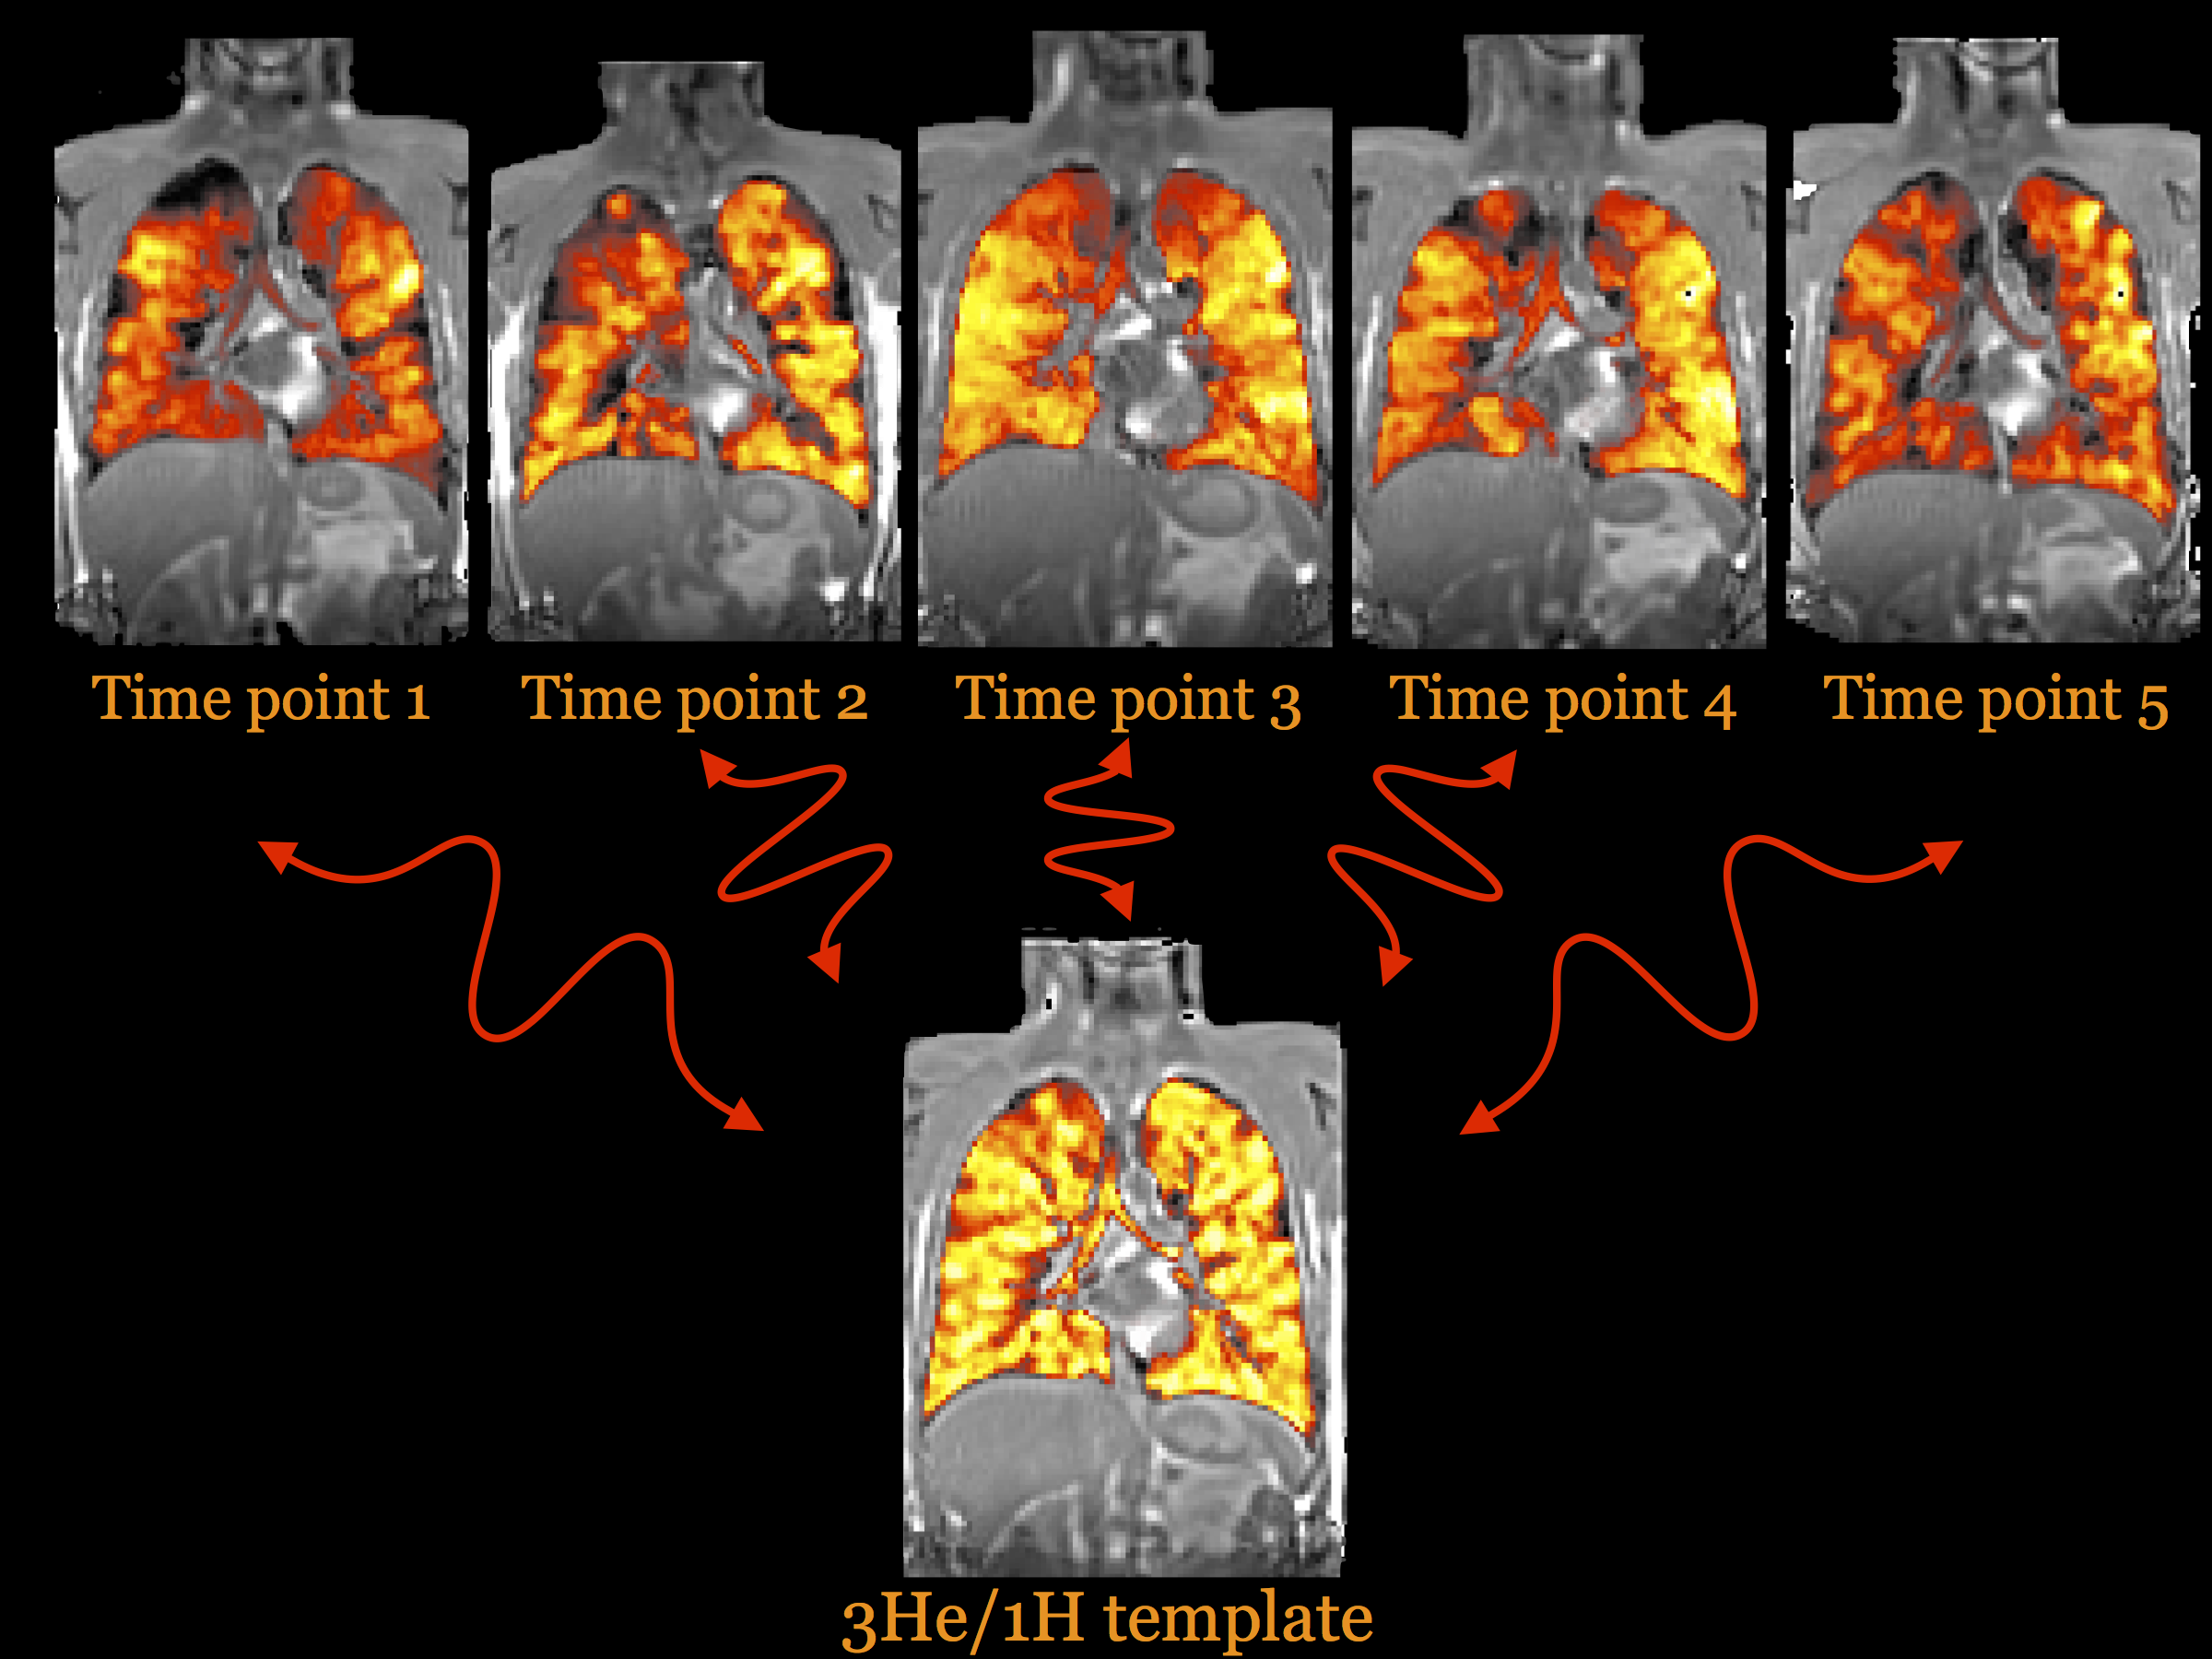
\includegraphics{Figures/H1He3Template.png}
\caption{Multivariate template construction using both 3He and 1H
images. To create a normalized patient-specific space for statistical
analysis of the longitudinal data, a template was created from the 3He
and 1H data from each of the 5 time points. Aligned results are shown of
the simultaneous acquisition by superimposing the faux color-rendered
3He image over the grayscale 1H image. The template was created
iteratively wherein the algorithm alternated between averaging the
registered images then registering each time point to the average image
(i.e., template estimate).}
\end{figure}

Eight patients completed the study. For every patient, a template was
created from the 3He and 1H data from each of the 5 time points to
provide a normalized patient-specific space for subsequent statistical
analysis of the longitudinal data. The template construction algorithm
described by Avants et al. {[}29{]} normally related to T1-weighted
brain data, was applied to the pulmonary data. The simultaneous
acquisition of the 3He and 1H MR images allowed multimodal processing
{[}30{]} in which both modalities were used to coordinate the data
processing to simultaneously produce 3He and 1H templates. This process
is illustrated in Figure 1 for a single patient. The alignment results
of the simultaneous acquisition are shown by overlaying the faux
color-rendered 3He image over the grayscale 1H image. The template was
generated iteratively wherein the algorithm alternated between averaging
the registered images then registering each time point to the average
image (i.e., template estimate).

\begin{figure}[htbp]
\centering
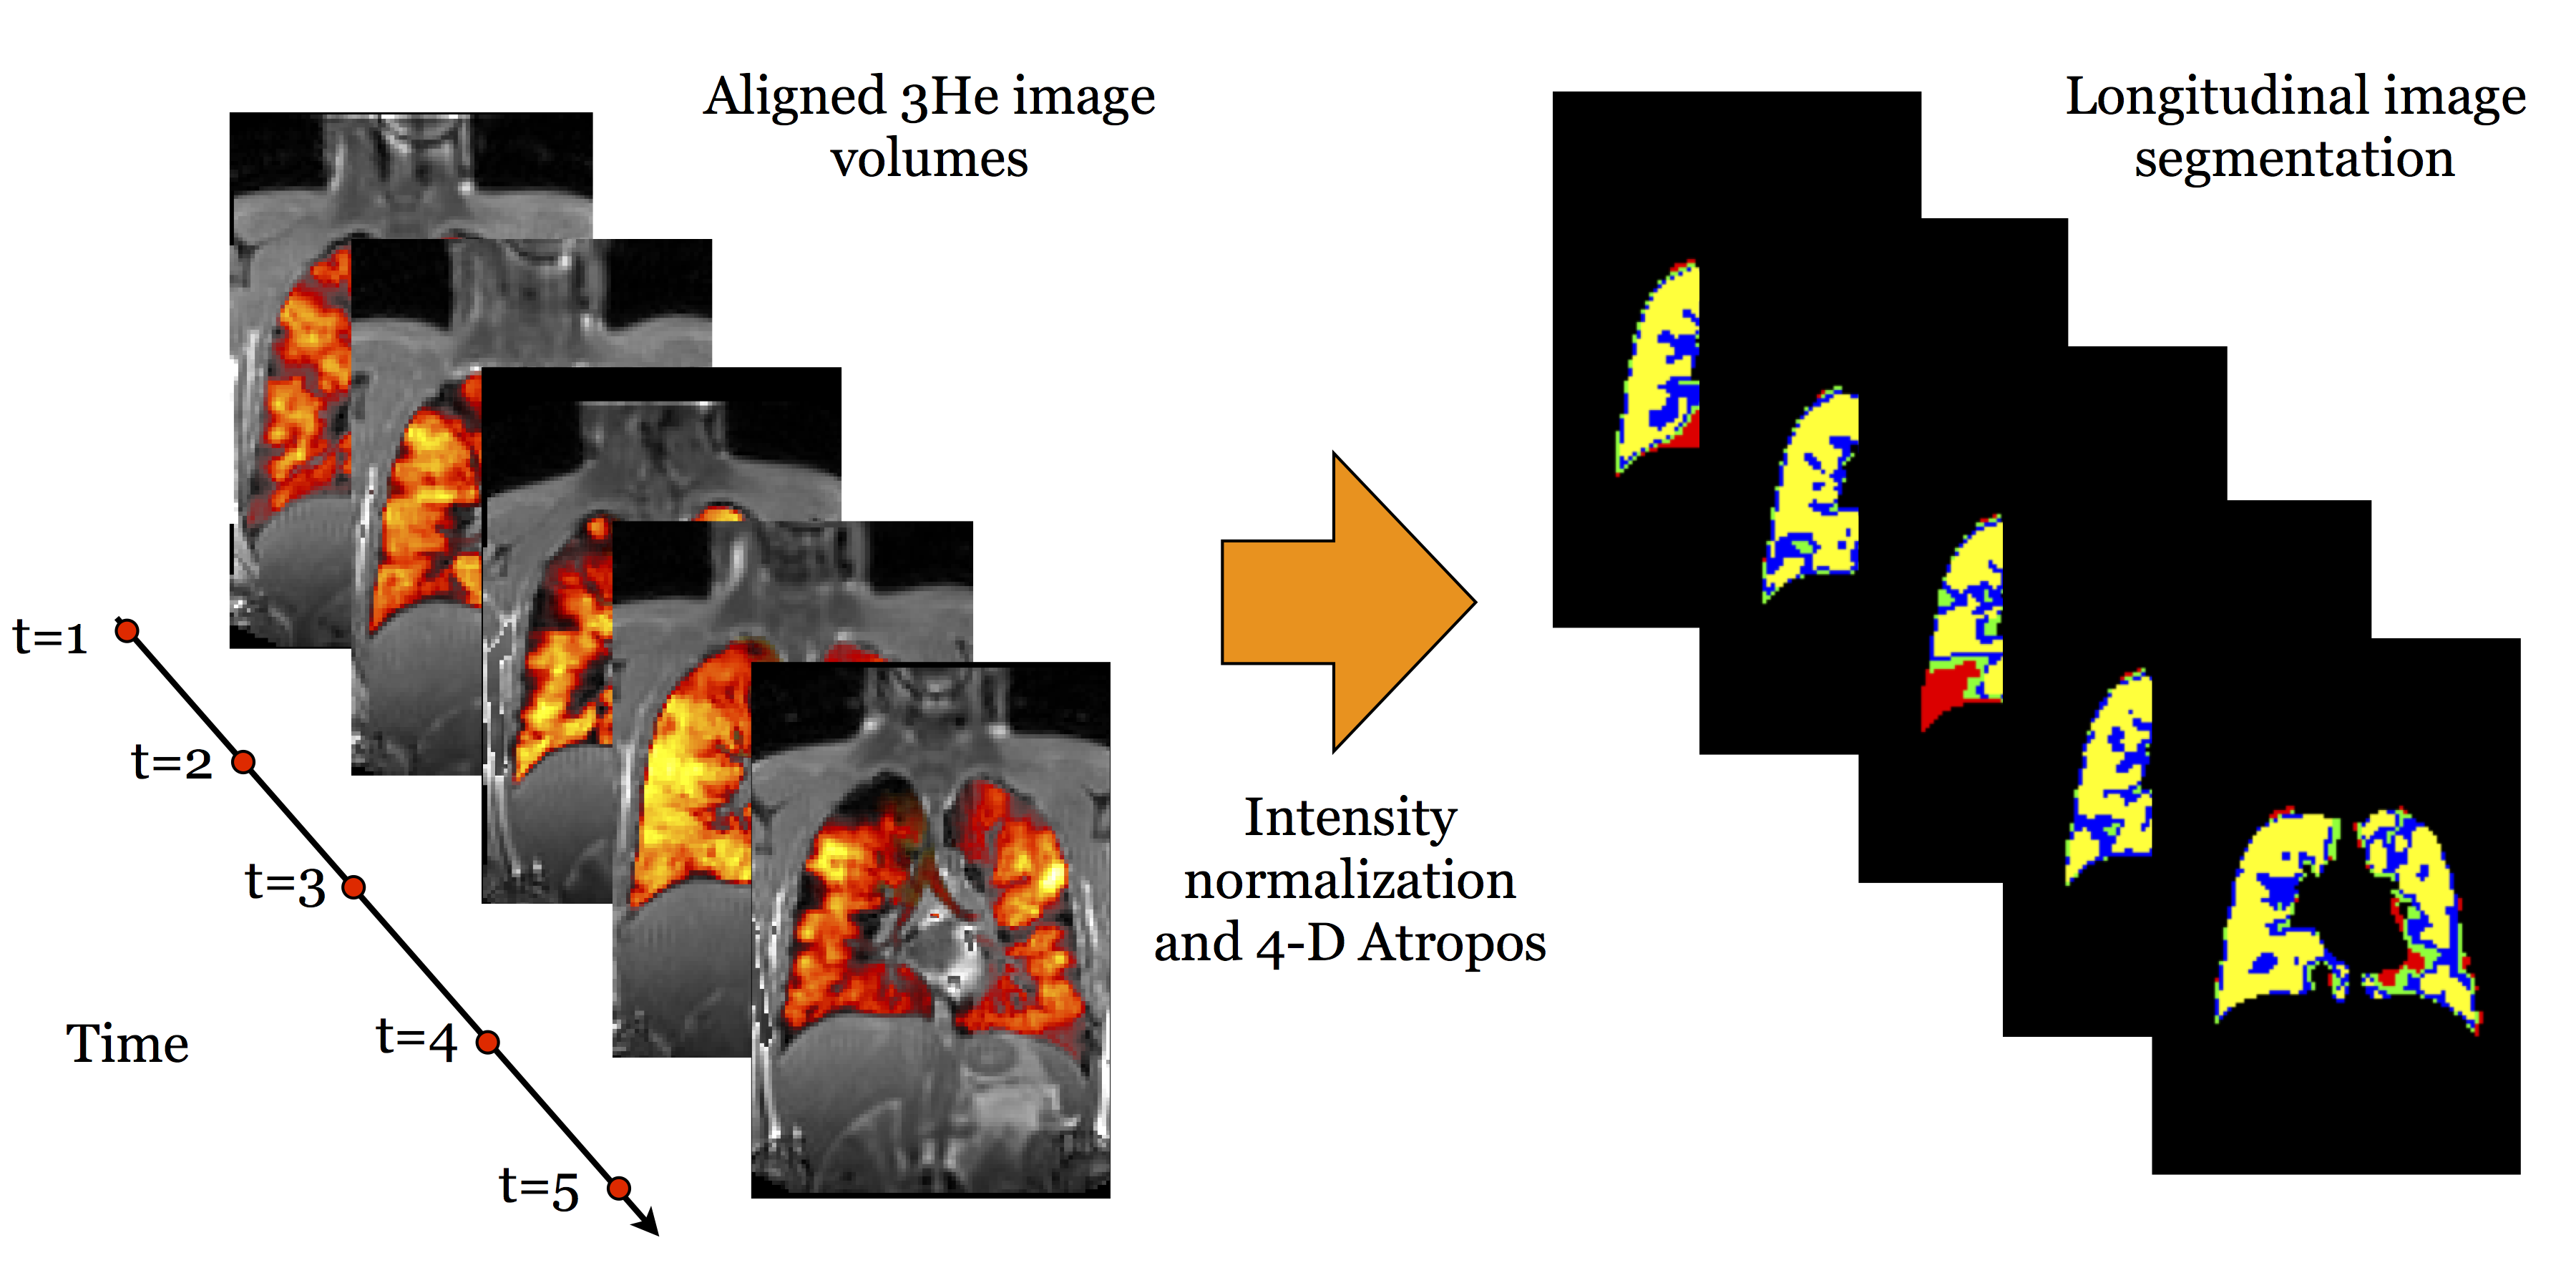
\includegraphics{Figures/4dSegmentation.png}
\caption{Four-dimensional (4-D) segmentation of the aligned 3-D image
volumes. After N4 inhomogeneity correction was applied to the 5 time
point image volumes, each of the corrected 3-D images from time points 2
through 5 were intensity normalized to the first time point. The 5
resulting corrected and normalized 3-D images were subsequently collated
into a single, 4-D spatio-temporal image, which was segmented into 4
classes using Atropos segmentation.}
\end{figure}

After N4 inhomogeneity correction was applied to each of the 5 time
point image volumes, the individual corrected 3-D images from time
points 2 through 5 were intensity normalized to the first time point.
The 5 resulting corrected and normalized 3-D images were then collated
into a single, 4-D spatio-temporal image, which was segmented using
Atropos into 4 classes (Figure 2).

\begin{figure}[htbp]
\centering
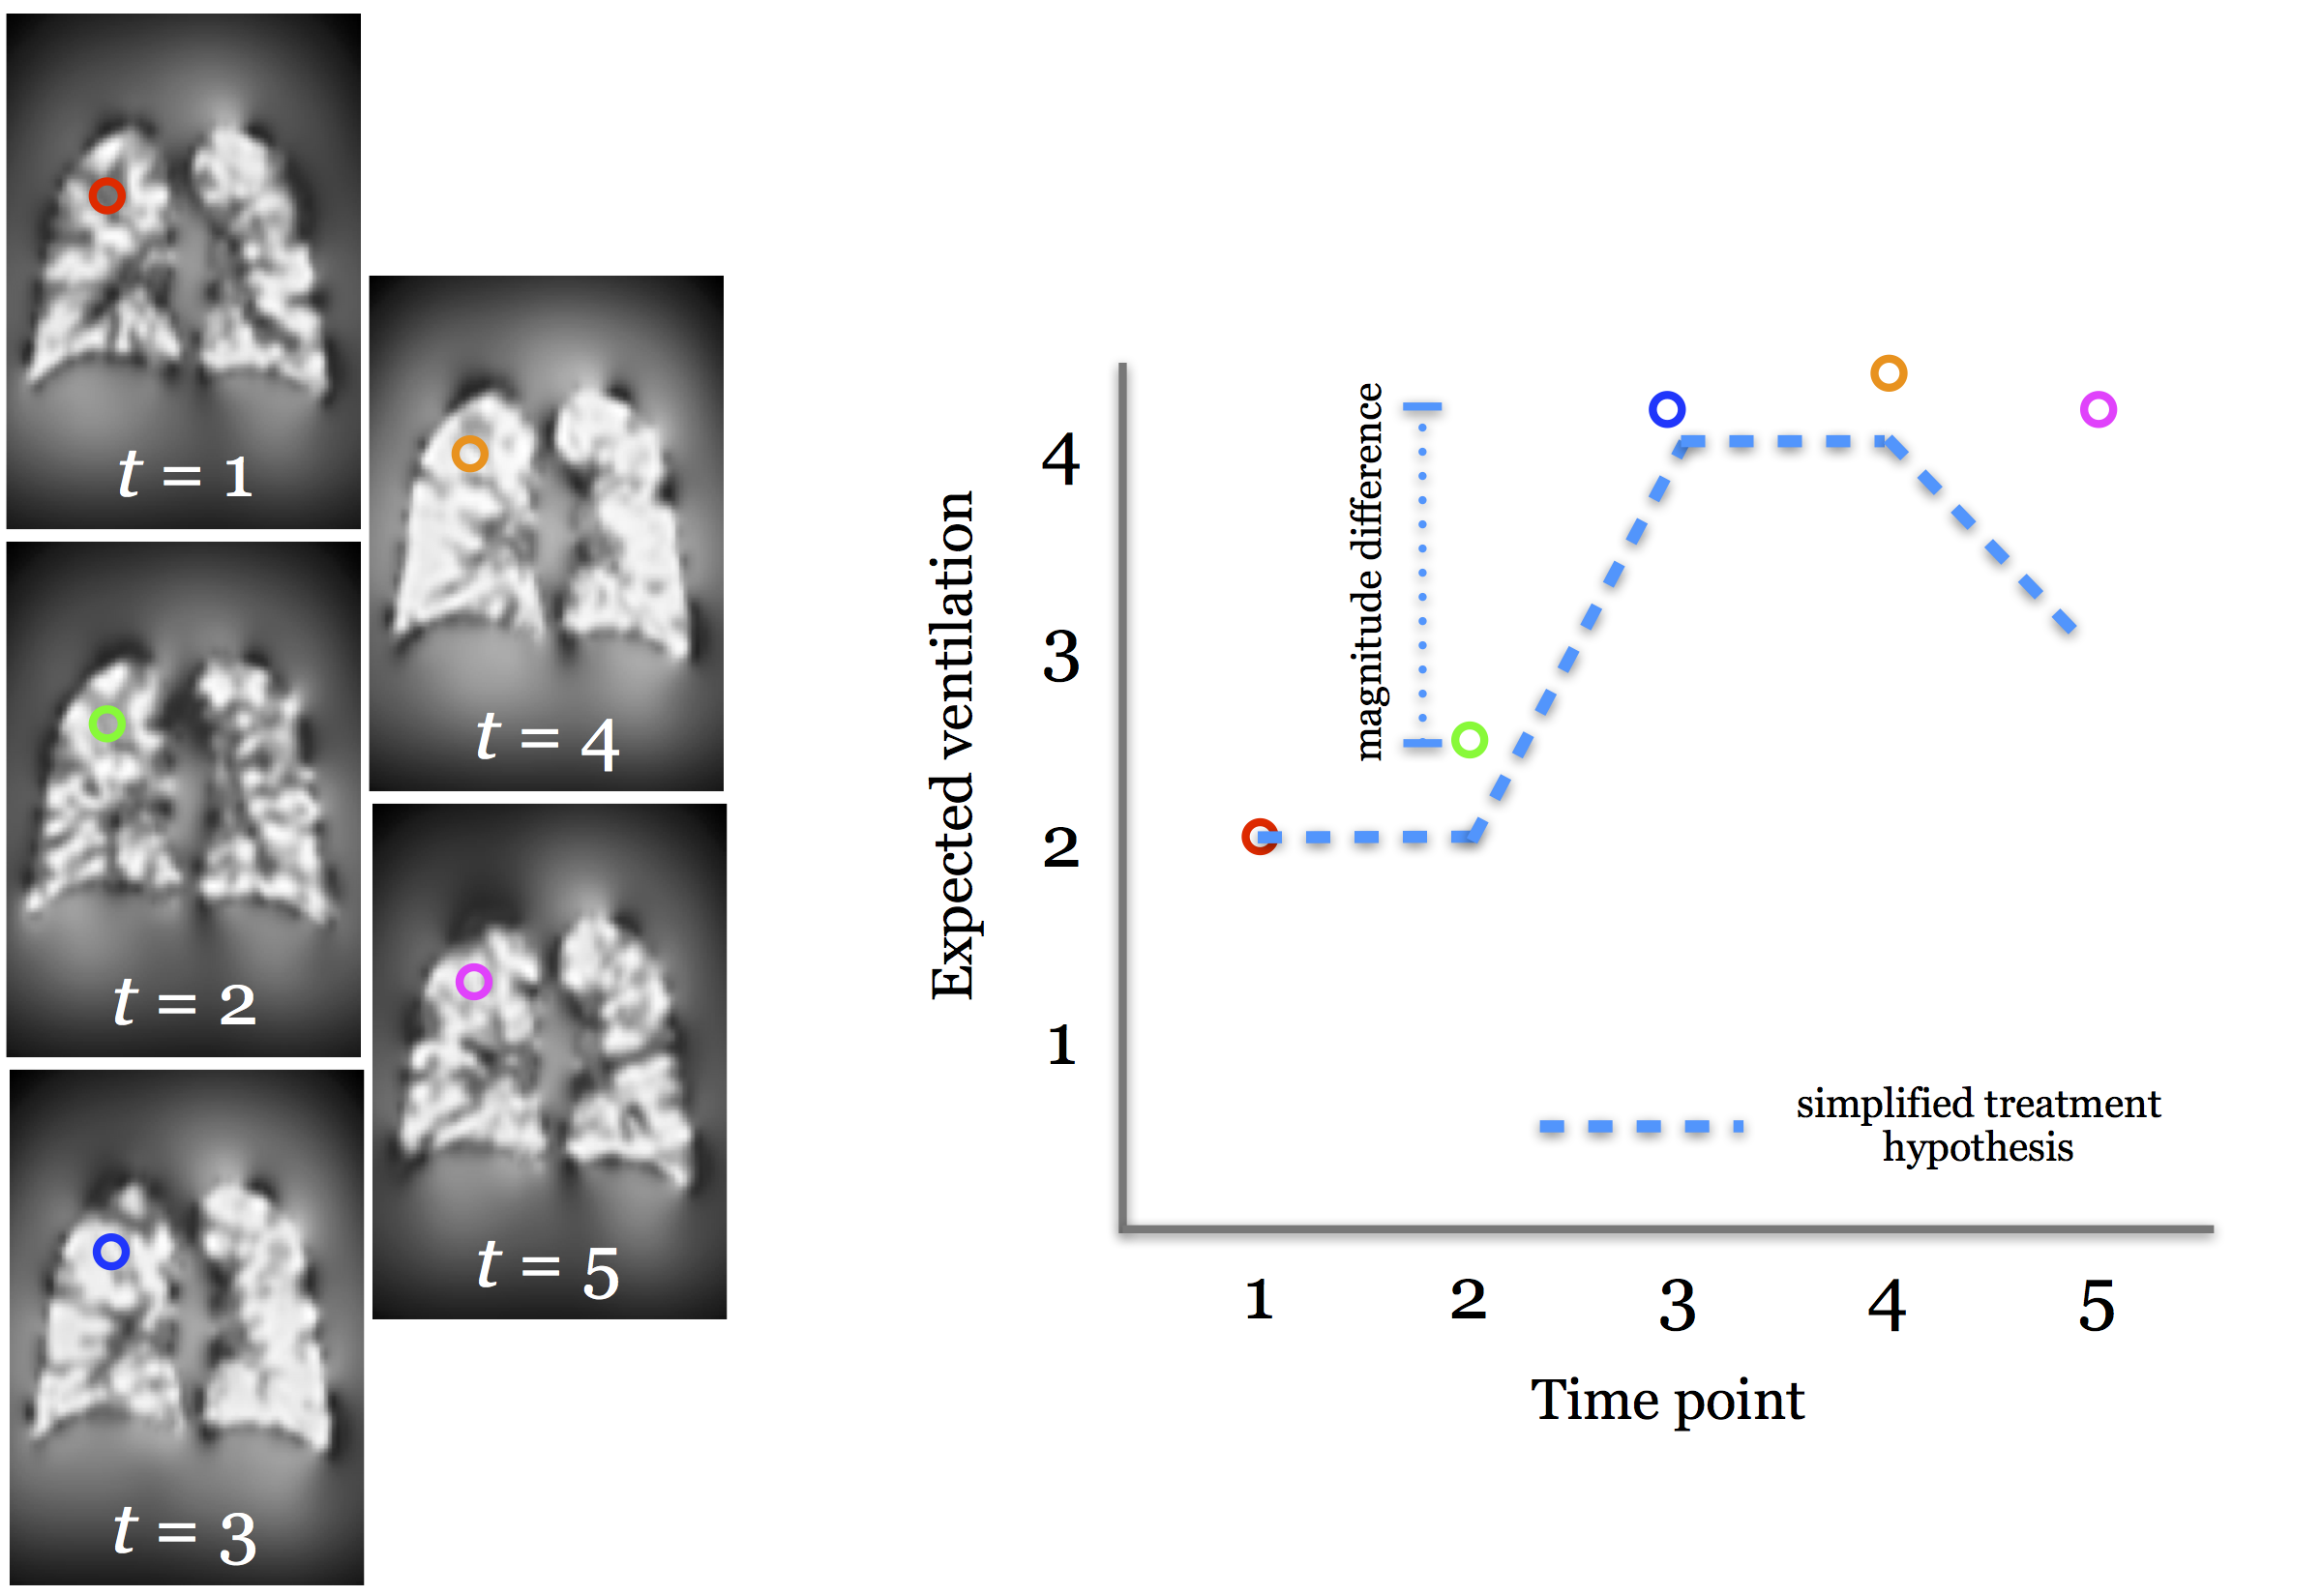
\includegraphics{Figures/correlation.png}
\caption{Voxelwise regression analysis to determine image-based response
to treatment. Treatment effects are expected to follow the simplified
treatment hypothesis illustrated with the dashed blue line in the plot
on the right. To explore how the longitudinal change in expected
ventilation follows this treatment hypothesis with image data, the
aligned expected ventilation maps were smoothed (to account for
potential voxelwise misalignments), and regression of voxelwise
intensities with the simplified treatment hypothesis was quantified.}
\end{figure}

Following inhomogeneity correction and segmentation of the longitudinal
image volumes for each of the 8 patients, expected ventilation image
maps were created from the segmentation output using Equation 4. Images
were then smoothed, as demonstrated in Figure 3, to account for any
registration inaccuracies. A volumetric correlation map was generated
for each of the 8 patients by identifying positively and negatively
correlated regions satisfying \(|r| \geq 0.5\) and
\(|EV_{3} - EV_{2}| \geq 0.1\), wherein \(r\) is Pearson's correlation
coefficient, and \(EV_{3}\) and \(EV_{2}\) are the expected ventilation
values at time points 3 and 2, respectively. In the relevant correlation
map for each patient (Figure 4), orange and blue differentiate the
positively and negatively correlated regions, respectively. Subsequent
analyses included the calculation of positively and negatively
correlated subvolumes in the template space (Table 1) to provide a
global synthesis of the region-based quantities. Furthermore, regions of
the lung that improved with treatment could be identified in a
patient-specific manner. For example, in Figure 5, a view of the left
lung of patient 3 can be seen, showing only positively correlated
regions. The arrows designate the lobar fissure, revealing a predominant
upper lobe treatment effect in this particular patient.

\begin{figure}[htbp]
\centering
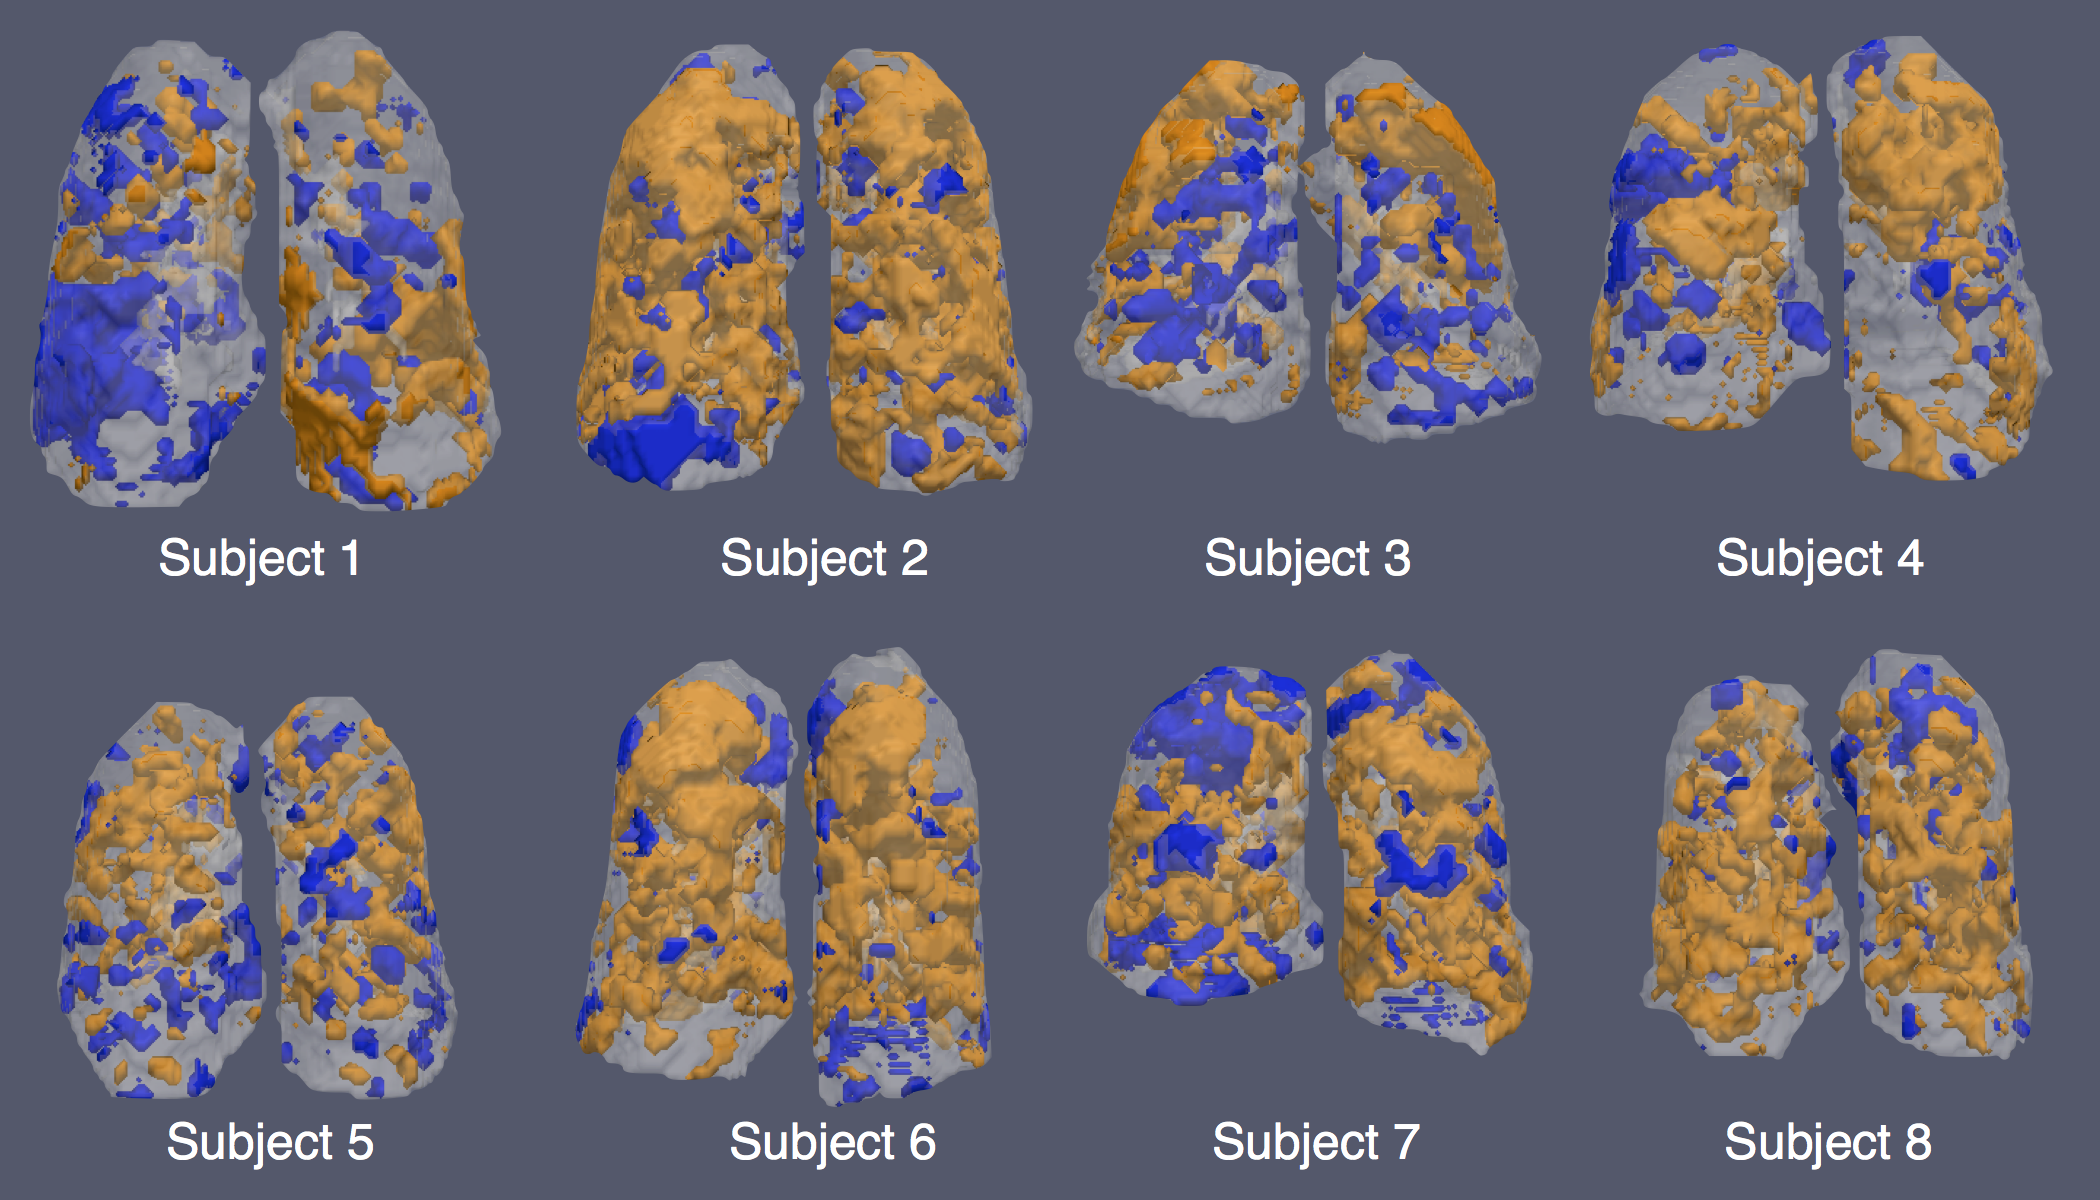
\includegraphics{Figures/3Dcorrelations.png}
\caption{Signed magnitude maps for all 8 patients showing regions of
significant positive (orange) and negative (blue) correlations, i.e.,
regions that responded according to the treatment hypothesis appear in
orange, whereas regions exhibiting inverse correlations appear in blue.
The rendered regions had absolute correlation values greater than or
equal to 0.5 and an effect size (i.e., the difference in expected
ventilation between time points \(t=2\) and \(t=3\)) greater than or
equal to 1.0.}
\end{figure}

\begin{table}[!htb]
  \centering
 \caption{Summary statistics for the correlation volumes shown in Figure 4.
          Given are total volume and positively and negatively correlated subvolumes.
          }
  \begin{tabular*}{0.8\textwidth}{@{\extracolsep{\fill}} crrr}
    \toprule
    \multicolumn{1}{c}{\textbf{Subject}} & \multicolumn{1}{c}{\textbf{Volume (L)}} &
    \multicolumn{1}{c}{\specialcell{\textbf{Positively Correlated}\\\textbf{Subvolume (L)}}}  &
    \multicolumn{1}{c}{\specialcell{\textbf{Negatively Correlated}\\\textbf{Subvolume (L)}}}\\
    \toprule
    1 & 3.52 & 0.73 & 0.62 \\
    \midrule
    2 & 5.56 & 2.95 & 0.46 \\
    \midrule
    3 & 4.70 & 1.32 & 0.93 \\
    \midrule
    4 & 5.05 & 1.76 & 0.55 \\
    \midrule
    5 & 3.82 & 1.11 & 0.39 \\
    \midrule
    6 & 4.60 & 2.11 & 0.32 \\
    \midrule
    7 & 4.44 & 1.57 & 0.75 \\
    \midrule
    8 & 3.86 & 1.58 & 0.32 \\
    \bottomrule
  \end{tabular*}
 \label{table:indices}
\end{table}




\begin{figure}[htbp]
\centering
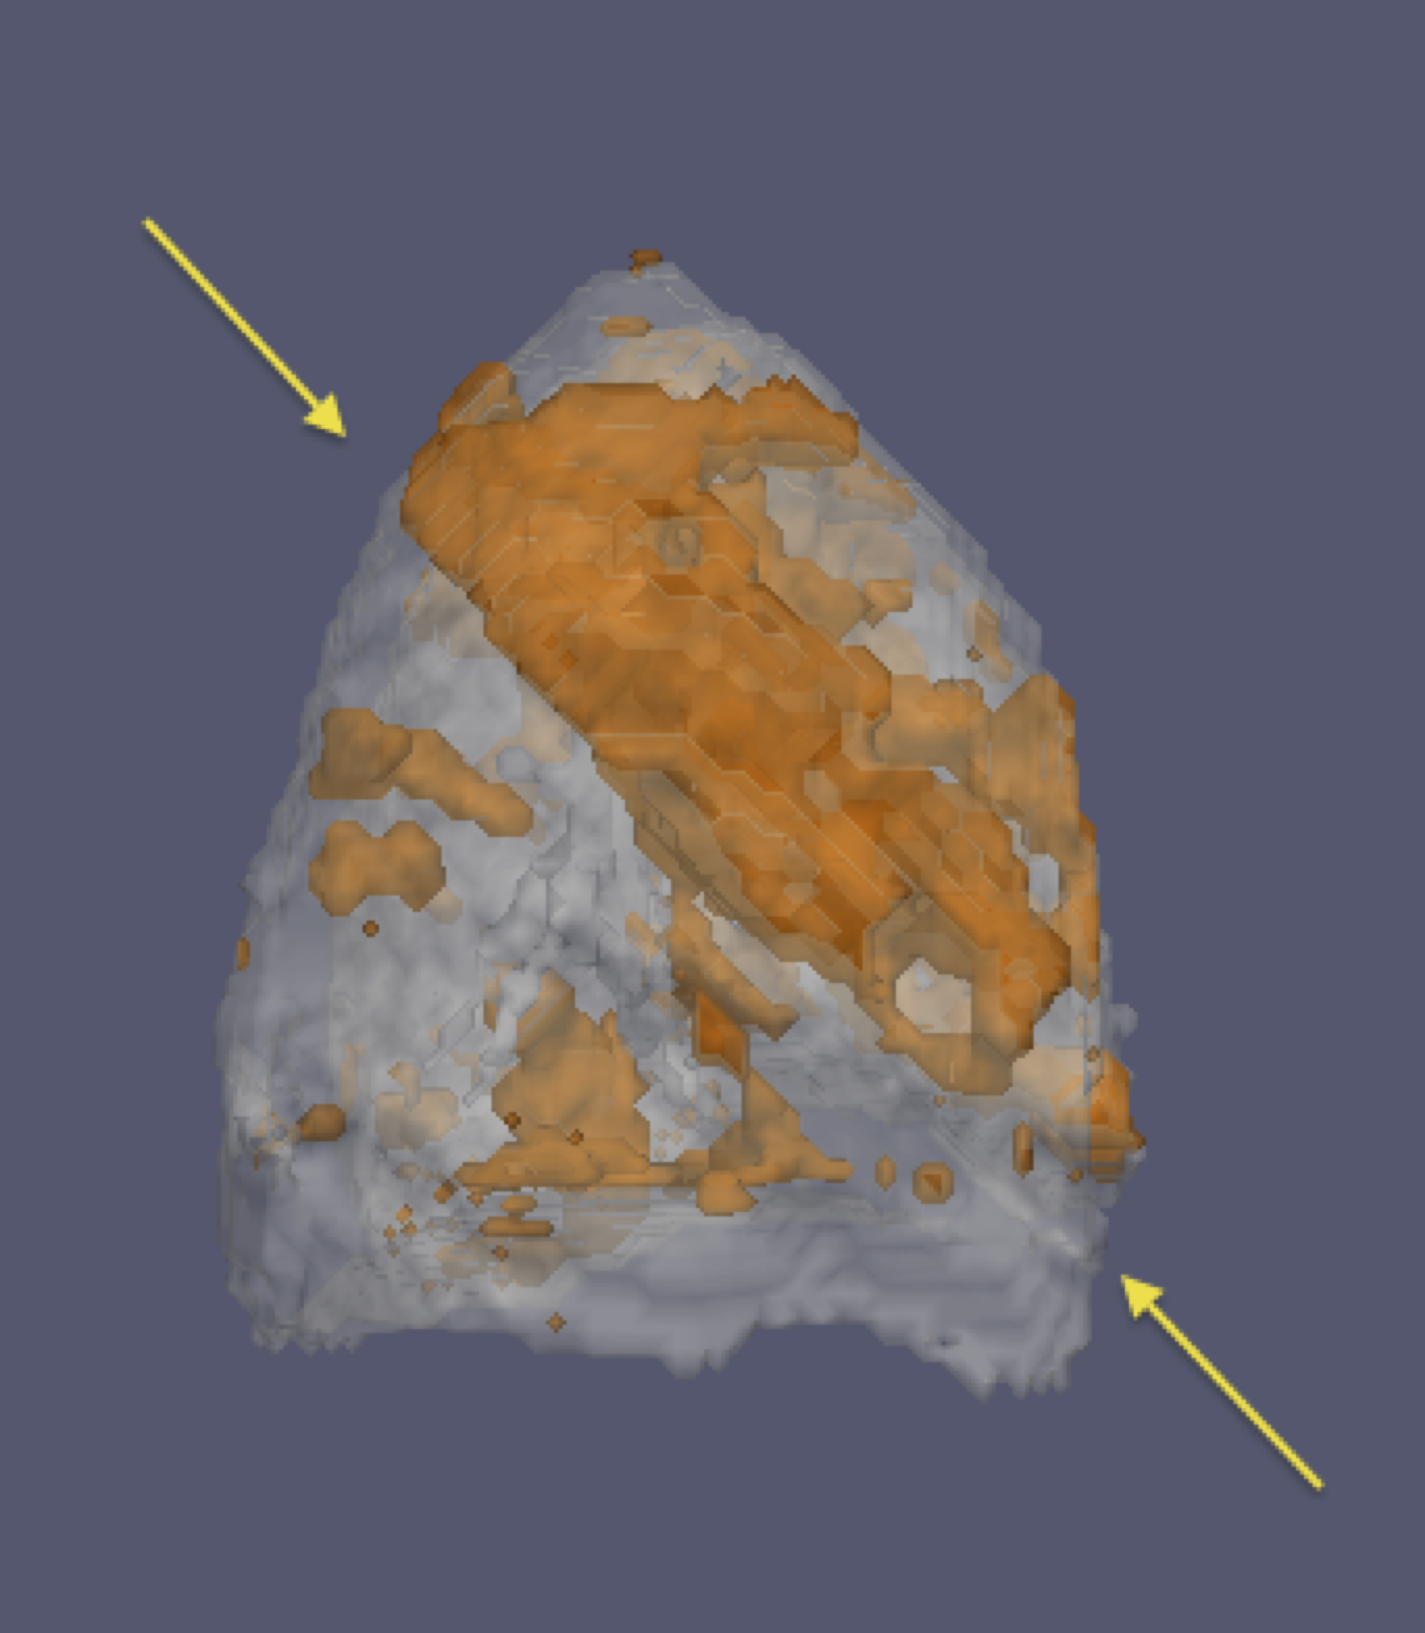
\includegraphics{Figures/subject3_stillframe63_lobe.png}
\caption{View of the left lung of patient 3, showing only positively
correlated regions (i.e., regions that improved with treatment). The
arrows indicate the lobar fissure, demonstrating a predominant upper
lobe treatment effect.}
\end{figure}

\section{Discussion}\label{discussion}

Increased use of imaging for pulmonary longitudinal studies will require
computational techniques to quantify and visualize spatial data in both
local and global terms. A framework has been presented here for data
preparation in future single-patient longitudinal studies whereby
multivariate template construction results in longitudinal alignment.
Results were presented using a unique cohort of patients with CF imaged
at 5 discrete time points while undergoing various stages of drug
treatment.

For the analysis of this work, patient-specific templates were generated
directly from the image data. Given the variability in lung shape across
populations and the lack of publicly available lung atlases, generating
population- or patient-specific templates enhanced the accuracy of the
longitudinal analysis. Furthermore, the voxel-based longitudinal
analysis technique used in this study enables voxelwise statistical
regression for determining spatial correlation with expected treatment
effects. This provides a new visualization and quantitative technique
for exploring clinical hypotheses regarding changes in lung function.

In conclusion, these preliminary results demonstrate the potential
utility of the proposed framework for providing regional information
concerning such pulmonary research topics as disease progression or
response to treatment. The preprocessing steps of template building,
intensity normalization, inhomogeneity correction, and segmentation are
all available in the ANTs distribution. Furthermore, the R statistical
project, which was used to perform statistical analysis, is available at
www.r-project.org. Hence, the processing pipeline is readily available
as an open source of information to researchers who desire to
participate in and extend this work.

\clearpage

\subsection{Acknowledgments}\label{acknowledgments}

Vertex Pharmaceuticals Incorporated provided funding for editorial
support in the development of this manuscript; Edwin Thrower, PhD,
provided editorial support and Dena McWain of Infusion Communications
copyedited and styled the manuscript per journal requirements. Vertex
Pharmaceuticals Incorporated reviewed and provided feedback on the
manuscript to the authors. The authors had full editorial control of the
manuscript and provided their final approval of all content.

~~

\subsection{Author Disclosures}\label{author-disclosures}

Nicholas J. Tustison:

Benjamin Contrella:

Talissa A. Altes:

Brian B. Avants:

Eduard E. de Lange:

John P. Mugler III:

\clearpage

\section*{References}\label{references}
\addcontentsline{toc}{section}{References}

\hypertarget{refs}{}
\hypertarget{ref-Burchfiel:1995aa}{}
1. Burchfiel, C. M., Marcus, E. B., Curb, J. D., Maclean, C. J.,
Vollmer, W. M., Johnson, L. R., Fong, K. O., Rodriguez, B. L., Masaki,
K. H., and Buist, A. S. ``\textbf{Effects of Smoking and Smoking
Cessation on Longitudinal Decline in Pulmonary Function}'' \emph{Am J
Respir Crit Care Med} 151, no. 6 (1995): 1778--85.
doi:\href{https://doi.org/10.1164/ajrccm.151.6.7767520}{10.1164/ajrccm.151.6.7767520}

\hypertarget{ref-Kanner:1999aa}{}
2. Kanner, R. E., Connett, J. E., Williams, D. E., and Buist, A. S.
``\textbf{Effects of Randomized Assignment to a Smoking Cessation
Intervention and Changes in Smoking Habits on Respiratory Symptoms in
Smokers with Early Chronic Obstructive Pulmonary Disease: The Lung
Health Study}'' \emph{Am J Med} 106, no. 4 (1999): 410--6.

\hypertarget{ref-Sears:2003aa}{}
3. Sears, M. R., Greene, J. M., Willan, A. R., Wiecek, E. M., Taylor, D.
R., Flannery, E. M., Cowan, J. O., Herbison, G. P., Silva, P. A., and
Poulton, R. ``\textbf{A Longitudinal, Population-Based, Cohort Study of
Childhood Asthma Followed to Adulthood}'' \emph{N Engl J Med} 349, no.
15 (2003): 1414--22.
doi:\href{https://doi.org/10.1056/NEJMoa022363}{10.1056/NEJMoa022363}

\hypertarget{ref-Schultz:2016aa}{}
4. Schultz, E. S., Hallberg, J., Bellander, T., Bergström, A., Bottai,
M., Chiesa, F., Gustafsson, P. M., Gruzieva, O., Thunqvist, P.,
Pershagen, G., and Melén, E. ``\textbf{Early-Life Exposure to
Traffic-Related Air Pollution and Lung Function in Adolescence}''
\emph{Am J Respir Crit Care Med} 193, no. 2 (2016): 171--7.
doi:\href{https://doi.org/10.1164/rccm.201505-0928OC}{10.1164/rccm.201505-0928OC}

\hypertarget{ref-Langley:2005aa}{}
5. Langley, S. J., Goldthorpe, S., Craven, M., Woodcock, A., and
Custovic, A. ``\textbf{Relationship Between Exposure to Domestic
Allergens and Bronchial Hyperresponsiveness in Non-Sensitised, Atopic
Asthmatic Subjects}'' \emph{Thorax} 60, no. 1 (2005): 17--21.
doi:\href{https://doi.org/10.1136/thx.2004.027839}{10.1136/thx.2004.027839}

\hypertarget{ref-Greenwald:1987aa}{}
6. Greenwald, G. I., Tashkin, D. P., Gong, H., Simmons, M., Duann, S.,
Furst, D. E., and Clements, P. ``\textbf{Longitudinal Changes in Lung
Function and Respiratory Symptoms in Progressive Systemic Sclerosis.
Prospective Study}'' \emph{Am J Med} 83, no. 1 (1987): 83--92.

\hypertarget{ref-Love:1982aa}{}
7. Love, R. G. and Miller, B. G. ``\textbf{Longitudinal Study of Lung
Function in Coal-Miners}'' \emph{Thorax} 37, no. 3 (1982): 193--7.

\hypertarget{ref-Rom:1992aa}{}
8. Rom, W. N. ``\textbf{Accelerated Loss of Lung Function and Alveolitis
in a Longitudinal Study of Non-Smoking Individuals with Occupational
Exposure to Asbestos}'' \emph{Am J Ind Med} 21, no. 6 (1992): 835--44.

\hypertarget{ref-Sherman:1992aa}{}
9. Sherman, C. B., Xu, X., Speizer, F. E., Ferris, B. G., Jr, Weiss, S.
T., and Dockery, D. W. ``\textbf{Longitudinal Lung Function Decline in
Subjects with Respiratory Symptoms}'' \emph{Am Rev Respir Dis} 146, no.
4 (1992): 855--9.
doi:\href{https://doi.org/10.1164/ajrccm/146.4.855}{10.1164/ajrccm/146.4.855}

\hypertarget{ref-Vestbo:2008aa}{}
10. Vestbo, J., Anderson, W., Coxson, H. O., Crim, C., Dawber, F.,
Edwards, L., Hagan, G., Knobil, K., Lomas, D. A., MacNee, W., Silverman,
E. K., Tal-Singer, R., and ECLIPSE investigators. ``\textbf{Evaluation
of COPD Longitudinally to Identify Predictive Surrogate End-Points
(ECLIPSE)}'' \emph{Eur Respir J} 31, no. 4 (2008): 869--73.
doi:\href{https://doi.org/10.1183/09031936.00111707}{10.1183/09031936.00111707}

\hypertarget{ref-Ohara:2008aa}{}
11. Ohara, T., Hirai, T., Sato, S., Terada, K., Kinose, D., Haruna, A.,
Marumo, S., Nishioka, M., Ogawa, E., Nakano, Y., Hoshino, Y., Ito, Y.,
Matsumoto, H., Niimi, A., Mio, T., Chin, K., Muro, S., and Mishima, M.
``\textbf{Longitudinal Study of Airway Dimensions in Chronic Obstructive
Pulmonary Disease Using Computed Tomography}'' \emph{Respirology} 13,
no. 3 (2008): 372--8.
doi:\href{https://doi.org/10.1111/j.1440-1843.2008.01269.x}{10.1111/j.1440-1843.2008.01269.x}

\hypertarget{ref-Dirksen:1999aa}{}
12. Dirksen, A., Dijkman, J. H., Madsen, F., Stoel, B., Hutchison, D.
C., Ulrik, C. S., Skovgaard, L. T., Kok-Jensen, A., Rudolphus, A.,
Seersholm, N., Vrooman, H. A., Reiber, J. H., Hansen, N. C., Heckscher,
T., Viskum, K., and Stolk, J. ``\textbf{A Randomized Clinical Trial of
Alpha(1)-Antitrypsin Augmentation Therapy}'' \emph{Am J Respir Crit Care
Med} 160, no. 5 Pt 1 (1999): 1468--72.
doi:\href{https://doi.org/10.1164/ajrccm.160.5.9901055}{10.1164/ajrccm.160.5.9901055}

\hypertarget{ref-Remy-Jardin:2002aa}{}
13. Remy-Jardin, M., Edme, J.-L., Boulenguez, C., Remy, J., Mastora, I.,
and Sobaszek, A. ``\textbf{Longitudinal Follow-up Study of Smoker's Lung
with Thin-Section CT in Correlation with Pulmonary Function Tests}''
\emph{Radiology} 222, no. 1 (2002): 261--70.
doi:\href{https://doi.org/10.1148/radiol.2221001154}{10.1148/radiol.2221001154}

\hypertarget{ref-Stolk:2003aa}{}
14. Stolk, J., Ng, W. H., Bakker, M. E., Reiber, J. H. C., Rabe, K. F.,
Putter, H., and Stoel, B. C. ``\textbf{Correlation Between Annual Change
in Health Status and Computer Tomography Derived Lung Density in
Subjects with Alpha1-Antitrypsin Deficiency}'' \emph{Thorax} 58, no. 12
(2003): 1027--30.

\hypertarget{ref-Parr:2008aa}{}
15. Parr, D. G., Sevenoaks, M., Deng, C., Stoel, B. C., and Stockley, R.
A. ``\textbf{Detection of Emphysema Progression in Alpha 1-Antitrypsin
Deficiency Using CT Densitometry; Methodological Advances}''
\emph{Respir Res} 9, (2008): 21.
doi:\href{https://doi.org/10.1186/1465-9921-9-21}{10.1186/1465-9921-9-21}

\hypertarget{ref-Stolk:2007aa}{}
16. Stolk, J., Putter, H., Bakker, E. M., Shaker, S. B., Parr, D. G.,
Piitulainen, E., Russi, E. W., Grebski, E., Dirksen, A., Stockley, R.
A., Reiber, J. H. C., and Stoel, B. C. ``\textbf{Progression Parameters
for Emphysema: A Clinical Investigation}'' \emph{Respir Med} 101, no. 9
(2007): 1924--30.
doi:\href{https://doi.org/10.1016/j.rmed.2007.04.016}{10.1016/j.rmed.2007.04.016}

\hypertarget{ref-Tanabe:2011aa}{}
17. Tanabe, N., Muro, S., Hirai, T., Oguma, T., Terada, K., Marumo, S.,
Kinose, D., Ogawa, E., Hoshino, Y., and Mishima, M. ``\textbf{Impact of
Exacerbations on Emphysema Progression in Chronic Obstructive Pulmonary
Disease}'' \emph{Am J Respir Crit Care Med} 183, no. 12 (2011): 1653--9.
doi:\href{https://doi.org/10.1164/rccm.201009-1535OC}{10.1164/rccm.201009-1535OC}

\hypertarget{ref-Soejima:2000aa}{}
18. Soejima, K., Yamaguchi, K., Kohda, E., Takeshita, K., Ito, Y.,
Mastubara, H., Oguma, T., Inoue, T., Okubo, Y., Amakawa, K., Tateno, H.,
and Shiomi, T. ``\textbf{Longitudinal Follow-up Study of Smoking-Induced
Lung Density Changes by High-Resolution Computed Tomography}'' \emph{Am
J Respir Crit Care Med} 161, no. 4 Pt 1 (2000): 1264--73.
doi:\href{https://doi.org/10.1164/ajrccm.161.4.9905040}{10.1164/ajrccm.161.4.9905040}

\hypertarget{ref-Lange:1999aa}{}
19. Lange, E. E. de, Mugler, J. P., 3rd, Brookeman, J. R., Knight-Scott,
J., Truwit, J. D., Teates, C. D., Daniel, T. M., Bogorad, P. L., and
Cates, G. D. ``\textbf{Lung Air Spaces: MR Imaging Evaluation with
Hyperpolarized 3He Gas}'' \emph{Radiology} 210, no. 3 (1999): 851--7.
doi:\href{https://doi.org/10.1148/radiology.210.3.r99fe08851}{10.1148/radiology.210.3.r99fe08851}

\hypertarget{ref-Tustison:2010aa}{}
20. Tustison, N. J., Altes, T. A., Song, G., Lange, E. E. de, Mugler, J.
P., 3rd, and Gee, J. C. ``\textbf{Feature Analysis of Hyperpolarized
Helium-3 Pulmonary MRI: A Study of Asthmatics Versus Nonasthmatics}''
\emph{Magn Reson Med} 63, no. 6 (2010): 1448--55.
doi:\href{https://doi.org/10.1002/mrm.22390}{10.1002/mrm.22390}

\hypertarget{ref-Tustison:2011aa}{}
21. Tustison, N. J., Avants, B. B., Flors, L., Altes, T. A., Lange, E.
E. de, Mugler, J. P., 3rd, and Gee, J. C. ``\textbf{Ventilation-Based
Segmentation of the Lungs Using Hyperpolarized (3)He MRI}'' \emph{J Magn
Reson Imaging} 34, no. 4 (2011): 831--41.
doi:\href{https://doi.org/10.1002/jmri.22738}{10.1002/jmri.22738}

\hypertarget{ref-Kirby:2012aa}{}
22. Kirby, M., Heydarian, M., Svenningsen, S., Wheatley, A., McCormack,
D. G., Etemad-Rezai, R., and Parraga, G. ``\textbf{Hyperpolarized 3He
Magnetic Resonance Functional Imaging Semiautomated Segmentation}''
\emph{Acad Radiol} 19, no. 2 (2012): 141--52.
doi:\href{https://doi.org/10.1016/j.acra.2011.10.007}{10.1016/j.acra.2011.10.007}

\hypertarget{ref-Ley:2004aa}{}
23. Ley, S., Zaporozhan, J., Morbach, A., Eberle, B., Gast, K. K.,
Heussel, C. P., Biedermann, A., Mayer, E., Schmiedeskamp, J., Stepniak,
A., Schreiber, W. G., and Kauczor, H.-U. ``\textbf{Functional Evaluation
of Emphysema Using Diffusion-Weighted 3Helium-Magnetic Resonance
Imaging, High-Resolution Computed Tomography, and Lung Function Tests}''
\emph{Invest Radiol} 39, no. 7 (2004): 427--34.

\hypertarget{ref-Kirby:2010aa}{}
24. Kirby, M., Mathew, L., Wheatley, A., Santyr, G. E., McCormack, D.
G., and Parraga, G. ``\textbf{Chronic Obstructive Pulmonary Disease:
Longitudinal Hyperpolarized (3)He MR Imaging}'' \emph{Radiology} 256,
no. 1 (2010): 280--9.
doi:\href{https://doi.org/10.1148/radiol.10091937}{10.1148/radiol.10091937}

\hypertarget{ref-Collins:1994aa}{}
25. Collins, D. L., Neelin, P., Peters, T. M., and Evans, A. C.
``\textbf{Automatic 3D Intersubject Registration of MR Volumetric Data
in Standardized Talairach Space}'' \emph{J Comput Assist Tomogr} 18, no.
2 (): 192--205.

\hypertarget{ref-Smith:2004aa}{}
26. Smith, S. M. ``\textbf{Overview of FMRI Analysis}'' \emph{Br J
Radiol} 77 Spec No 2, (2004): S167--75.
doi:\href{https://doi.org/10.1259/bjr/33553595}{10.1259/bjr/33553595}

\hypertarget{ref-Altes:2012aa}{}
27. Altes, T., Johnson, M., III, J. M., Miller, G. W., Flors, L., Mata,
J., Salinas, C., Tustison, N., Lee, P.-S., Song, T., Yen, K., Froh, D.,
and Botfield, M. ``\textbf{The Effect of Ivacaftor, an Investigational
CFTR Potentiator, on Hyperpolarized Noble Gas Magnetic Resonance Imaging
in Subjects with Cystic Fibrosis Who Have the G551D-CFTR Mutation}''
(2012): A2814--A2814.

\hypertarget{ref-Nyul:2000aa}{}
28. Nyúl, L. G., Udupa, J. K., and Zhang, X. ``\textbf{New Variants of a
Method of MRI Scale Standardization}'' \emph{IEEE Trans Med Imaging} 19,
no. 2 (2000): 143--50.
doi:\href{https://doi.org/10.1109/42.836373}{10.1109/42.836373}

\hypertarget{ref-Avants:2010aa}{}
29. Avants, B. B., Yushkevich, P., Pluta, J., Minkoff, D., Korczykowski,
M., Detre, J., and Gee, J. C. ``\textbf{The Optimal Template Effect in
Hippocampus Studies of Diseased Populations}'' \emph{Neuroimage} 49, no.
3 (2010): 2457--66.
doi:\href{https://doi.org/10.1016/j.neuroimage.2009.09.062}{10.1016/j.neuroimage.2009.09.062}

\hypertarget{ref-Tustison:2015aa}{}
30. Tustison, N. J., Shrinidhi, K. L., Wintermark, M., Durst, C. R.,
Kandel, B. M., Gee, J. C., Grossman, M. C., and Avants, B. B.
``\textbf{Optimal Symmetric Multimodal Templates and Concatenated Random
Forests for Supervised Brain Tumor Segmentation (Simplified) with
ANTsR}'' \emph{Neuroinformatics} 13, no. 2 (2015): 209--25.
doi:\href{https://doi.org/10.1007/s12021-014-9245-2}{10.1007/s12021-014-9245-2}

\end{document}
